\chapter{Layered Editor Architectures}
\label{chap:layeredArchs}
{\em *** Version: \today~ ***}



\bc
* fix gesture to edit Rendering, unless gesture becomes something special
* rendering or presentation? Rendering is more clear, but editing the rendering does not make sense. (maybe just explain)

HOE HEEFT PRE HIERMEE TE MAKEN? pre geeft geen berekening, maar alleen verband, dus zelfs als level i opgeleverd door pre, dan nog is het invoer

- Numbering 0 = doc, downwards like lines on a page.
** ?Add a $lower = EDIT~levels~gesture$ condition that states the result is what we mean with the gesture?



IMPORTANT there seems to be an invariant that for a j:  i>j, all mappings are correct 
  ..           ...       
 .  .    ..   .   .   .. 
.    ....  ...     ...  .
 no it's not asymmetric. find out more about this.
 maybe it's just that a level is never presented twice without intr, and vice versa

RENDERER IS SPECIAL, LOWER THING IS NOT A TREE, EXPLAIN THAT THIS CHAPTER ONLY HOLDS FOR HIGHER LAYERS


\ec



% intro

prev. chap. spec for layer but not edit and transform

Next chapter, we give Haskell for the combination

\section{Spec}

First by figures, then give spec.


?? Add arrow for intended gesture update?

\subsection{Connecting layers}

figure with in and out from prev. (hiding internal)

\begin{figure}\begin{small}\begin{center}\begin{center}
\epsfig{file=pics/eps/singleToMulti.eps, width=125mm}\end{center}
\caption{Blaa}\label{singleToMulti} 
\end{center}\end{small}\end{figure}

Now connect

need to remove one update: plaatje 3 layers, one layer

\begin{figure}\begin{small}\begin{center}\begin{center}
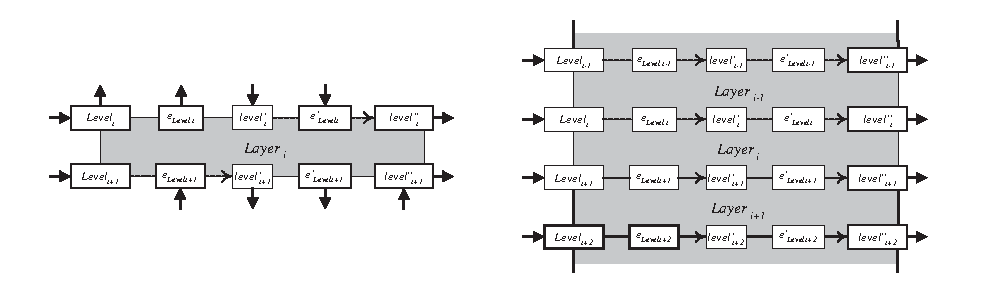
\epsfig{file=pics/eps/connectingLayers.eps, width=125mm}\end{center}
\caption{Blaa}\label{connectingLayers} 
\end{center}\end{small}\end{figure}



need something on top id
need something at bottom display and receive gesture. Also explain that user does not give e rendering

gesture depends on level, not edit. Also on other levels?


\begin{figure}\begin{small}\begin{center}\begin{center}
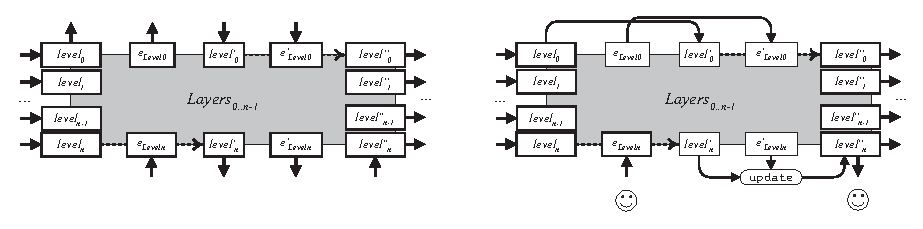
\epsfig{file=pics/eps/topAndBottom.eps, width=125mm}\end{center}
\caption{Blaa}\label{topAndBottom} 
\end{center}\end{small}\end{figure}


\subsection{Specifying connected layers}

First try: add i and leave out Edit and Transform

\begin{small}\( \begin{array}{lcl}  \label{inv:incrementality}
{\tt interpret_i}  ::  Sheet_{Intr,i} \rightarrow Level_{i+1} \rightarrow Level_{i} \rightarrow  Edit_{Level_{i+1}} \rightarrow Edit_{Core_{i}\times Info\idwn_{i}} \\
{\tt present_i}  ::  Sheet_{Pres,i} \rightarrow Level_{i} \rightarrow Level_{i+1}  \rightarrow Edit_{Level_{i}} \rightarrow Edit_{Core_{i+1}\times Info\iup_{i+1}}\\
\\
\end{array}\) \\
\( \begin{array}{rcll}  
level_{i+1} 	& = & Present_{i}~level_{i}						& \text{\{Precondition\}}\\
\\
level'_{i+1} 	& = & {\tt update}~e_{Level_{i+1}}~level_{i+1}                 & \text{\{Compute intermediate lower level\}}\\
e_{Core_{i} \times Info\idwn_{i}}  & = & {\tt interpret}_{i}~sheet_{Intr,i}~level_{i+1}~level_{i}~e_{Level_{i+1}} & \text{\{Compute higher core update\}}\\
e_{Level_{i}} & = & {\tt reuse}_{Intr,i}~level_{i}~e_{Core_{i}\times Info\idwn_{i}}     & \text{\{Reuse extra state\}}\\
level'_{i} & = & {\tt update}~e_{Level_{i}}~level_{i}                 & \text{\{Compute intermediate higher level\}}\\
\\\
level'_{i} & = & Interpret_{i}~level'_{i+1}						& \text{\{Intermediate condition\}}\\
\\
level''_{i} & = & {\tt update}~e'_{Level_{i}}~level'_{i}                 & \text{\{Compute final higher level\}}\\
e'_{Core_{i+1}\times Info\iup_{i+1}}  & = & {\tt present}_{i}~sheet_{Pres,i}~level'_{i}~level'_{i+1}~e'{Level_{i}} & \text{\{Compute new lower core\}}\\
e'_{Level_{i+1}} & = & {\tt reuse}_{Pres,i}~level_{i+1}~e'_{Core_{i+1}\times Info\iup_{i+1}} & \text{\{Reuse extra state\}}\\
level''_{i+1} & = & {\tt update}~e_{Level_{i+1}}~level_{i+1}                 & \text{\{Compute final lower level\}}\\
\\
level''_{i+1} & = & Present_{i}~level''_{i}						& \text{\{Postcondition\}}\\
\end{array}\)
\end{small}
\begin{center}(First try)\end{center}\vspace{1em}


level updates are double., so leave out one. intr leave out higher \{Compute intermediate higher level\} and pres leave out lower \{Compute final lower level\}. End up with:

\begin{small}\( \begin{array}{lcll} 
level'_{i+1} 	& = & {\tt update}~e_{Level_{i+1}}~level_{i+1}                 & \text{\{Compute intermediate lower level\}}\\
level''_{i} & = & {\tt update}~e'_{Level_{i}}~level'_{i}                 & \text{\{Compute final higher level\}}\\
\end{array}\)
\end{small}

Now we don't have computations for $level'_0$ and $level''{n}$. $e_n$ is not defined and $e'_0$


On top level, put the edit op back in, and just copy the not updated level:

\begin{small}\( \begin{array}{lcll} 
e'_{Level_{0}}  = e_{Level{0}}\\
level'_{0} =  level_{0}\\
\end{array}\)
\end{small}

On the bottom level, edit op comes from user. 

\begin{small}\( \begin{array}{lcll} 
e_{Level_{n}}  = EditGesture ??\\
level''_{n}  =  {\tt update}~e'_{Level_{n}}~level'_{n}\\
\end{array}\)
\end{small}


If we remove the double updates, and add the top and bottom stuff, we get a final specification:

\begin{itemize}
\item subscripts cannot be dropped anymore. Use data defs from prev chap (multiple layer perspective)
\item levels and layers mismatch, j and i
\item present, interpret, Sheet, all get i.  level,core,info h is level... i and level.. L is level.. i+1
\item update is generic, so no subscripts
\item only need one update on each layer, choose the source level because of inc comp. (ref to previous chap)
\item Edit and Transform disappear
\end{itemize}

Given level0..n for which Pres holds and an edit gesture, compute level''0..n so Pres holds again.

\begin{small}\( \begin{array}{lcl}  \label{inv:incrementality}
\text{\bf type}~Level_{0}  =  Core_{Intr,0} \times Extra_{Intr,0} \times Info\idwn_{0} \\
\text{\bf type}~Level_{n}  =  Core_{Pres,n} \times Extra_{Pres,n} \times  Info\iup_{n}\\
\lefteqn{\forall j:1 \le i \le n-1:}  \\
\text{\bf type}~Level_{j} =  Core_{Pres,j} \times Extra_{Pres,j}  \times Info\iup_{j}   
                                       =  Core_{Intr,j} \times Extra_{Intr,j} \times Info\idwn_{j}\\

e_{Level_{n}}  = EditGesture ??\\
e'_{Level_{0}}  = e_{Level{0}}\\
level'_{0} =  level_{0}\\
level''_{n}  =  {\tt update}~e'_{Level_{n}}~level'_{n}\\
\lefteqn{\forall i:0 \le i \le n-1:}  \\
{\tt interpret_i}  ::  Sheet_{Intr,i} \rightarrow Level_{i+1} \rightarrow Level_{i} \rightarrow  Edit_{Level_{i+1}} \rightarrow Edit_{Core_{i}\times Info\idwn_{i}} \\
{\tt present_i}  ::  Sheet_{Pres,i} \rightarrow Level_{i} \rightarrow Level_{i+1}  \rightarrow Edit_{Level_{i}} \rightarrow Edit_{Core_{i+1}\times Info\iup_{i+1}}\\
\\
\end{array}\) \\
\( \begin{array}{rcll}  
level_{i+1} 	& = & Present_{i}~level_{i}						& \text{\{Precondition\}}\\
\\
level'_{i+1} 	& = & {\tt update}~e_{Level_{i+1}}~level_{i+1}                 & \text{\{Compute intermediate lower level\}}\\
e_{Core_{i} \times Info\idwn_{i}}  & = & {\tt interpret}_{i}~sheet_{Intr,i}~level_{i+1}~level_{i}~e_{Level_{i+1}} & \text{\{Compute higher core update\}}\\
e_{Level_{i}} & = & {\tt reuse}_{Intr,i}~level_{i}~e_{Core_{i}\times Info\idwn_{i}}     & \text{\{Reuse extra state\}}\\
\\\
level'_{i} & = & Interpret_{i}~level'_{i+1}						& \text{\{Intermediate condition\}}\\
\\
level''_{i} & = & {\tt update}~e'_{Level_{i}}~level'_{i}                 & \text{\{Compute final higher level\}}\\
e'_{Core_{i+1}\times Info\iup_{i+1}}  & = & {\tt present}_{i}~sheet_{Pres,i}~level'_{i}~level'_{i+1}~e'{Level_{i}} & \text{\{Compute new lower core\}}\\
e'_{Level_{i+1}} & = & {\tt reuse}_{Pres,i}~level_{i+1}~e'_{Core_{i+1}\times Info\iup_{i+1}} & \text{\{Reuse extra state\}}\\
\\
level''_{i+1} & = & Present_{i}~level''_{i}						& \text{\{Postcondition\}}\\
\end{array}\)
\end{small}
\begin{center}(Final specification)\end{center}\vspace{1em}



\begin{itemize}
\item Starting the editor
\item level'' is level for next edit step
\item level for first needs to be initialized
\end{itemize}



%																
%																
%																
\section{}
\begin{itemize}
\item edit ops starting higher + es safety
\item tricky. maybe need to point out diff between skipping and processing
\end{itemize}

\section{}
\begin{itemize}
\item skipping cycles + es safety
\item ref to edit model
\end{itemize}

\section{Conclusions}














In this chapter, compose the layers from the previous chapter. First make a presentation system (not an editor), add layers. Then editor with layers. Finally, editor with the layers from previous chapter. And some more stuff for typical layer functionality. (skipping, and higher level edit ops)




%																
%																
%																
\section{Presentation system}

Presentation systems are applications that provide a user with some kind of view  on a data structure. Examples of presentation systems are pdf-viewers, image viewers, and web browsers, although the latter also have functionality for accessing non-local documents. Because an editor can be seen as  a presentation system with extra functionality  for editing the presented data, we will first develop a number of invariants that model the architecture of a presentation system, and in the next section rework the invariants to model an editor.


???
In this section, as well as in the following two, we will follow the same line of reasoning while constructing the invariants. First, we consider a simple case, in which the rendering of a document is computed in one single step. Secondly, the functions mapping the document to the rendering and the functions that map the edit gestures on the rendering to document updates are split in a number of subfunctions, each handling a specific step in the mapping process. And finally, we will extend the invariant to support the local state that was mentioned in the previous section. In some cases, a first attempt is given for the invariant, which is refined afterwards. 
??


%																
\subsection{Single stage presentation}

Suppose that there is a function $present :: Document \rightarrow Rendering$ that maps a $document$ of type $Document$ to a $rendering$ of type $Rendering$. We formally define the relation between the document and the rendering with the invariant:

\begin{small}
\bigskip \noindent
\xymatrix{
\data{$document$}\ar[d]	\\
\component{$present$} \ar[d] \\
\data{$rendering$}	 \\
}
\end{small}

\begin{small}\begin{align*}
present & :: Document \rightarrow Rendering \\
\end{align*}
\begin{math}
rendering = present~document
\hfill \text{\{Compute Rendering\}}
\end{math}\end{small}

{\centering (Invariant 2: One stage presentation, Final)\\}\vspace{1em}


%																
\subsection{Layered presentation}


\begin{small}
\bigskip \noindent
\xymatrix{
 \data{$level_{0}$}\ar[d]  \\
\component{$present_{0}$} \ar[d]\\
\data{$level_{1}$} \ar@{.>}[dd]   \\
		\\
\data{$level'_{n-1}$}\ar[d]	\\
\component{$present_{n-1}$} \ar[d]\\
\data{$level_{n}$}\\
}
\end{small}



\begin{small}
\begin{align*} % \label{lpupdate}
present_i & :: Level_i \rightarrow Level_{i+1} \\
\end{align*}
\begin{math}
\forall 0 \le i \le n-1: \\
level_0 = document \\
level_{i+1} = present_i~level_i\\
rendering = level_n \hfill \text{\{Compute Rendering\}}
\end{math}\end{small}

{\centering (Invariant 4: Layered presentation, Final)\\}\vspace{1em} 


%																
\subsection{Layered presentation with local state}


\begin{small}\begin{align*} % \label{llp}
present_i & :: Sheet_i \rightarrow Level_i \rightarrow Level_{i+1}\\
\end{align*}
\begin{math}
\forall 0 \le i \le n-1: \\
level_{i+1} = present_i~sheet_i~level_i
\hfill \text{\{Compute Rendering\}}
\end{math}\end{small}

{\centering (Invariant 5: Layered presentation with local state)\\}\vspace{1em}



\begin{figure}
\begin{small}
\begin{center}
\begin{center}
\end{center}\caption{ The edit process}\label{editprocess} 
\end{center}
\end{small}
\end{figure}


%																
%																
%																
\section{Editor}

plaatje van edit proces, show get gesture, update ...


%																
\subsection{Single stage editor}


\begin{small}
\bigskip \noindent
\xymatrix{
\data{$document$}\ar[d]	& 			& \data{$document'$}\ar[r] 		& \data{$document''$}\ar[d]  \\
\component{$present$} \ar[d] &			& \component{$interpret$} \ar[u]	& \component{$present$} \ar[d]\\
\data{$rendering$} \ar[r]	& \component{update} \ar[r] 	& \data{$rendering'$}\ar[u] 		& \data{$rendering''$}  \\
			& \data{$gesture$} \ar[u]	&				& 	 	
}
\end{small}




\begin{small}\begin{align*}% \label{sse}
update & :: Edit_\alpha \rightarrow \alpha \rightarrow \alpha \\
present & :: Document \rightarrow Rendering \\
interpret & :: Rendering \rightarrow Document \\
\end{align*} 
\begin{math}
rendering = present~document	\hfill \text{\{Precondition\}} \\
rendering' = update~gesture~rendering	\hfill \text{\{Update rendering\}} \\
document' = interpret~rendering' 	\hfill \text{\{Compute updated document\}}\\
document'' = document'		\\% \hfill \text{\{Update Document\}} \\
rendering'' = present~document''	\hfill \text{\{Postcondition + Compute rendering'\}} \\
\end{math}\end{small}
{\centering (Invariant 6: One stage editor, 1st attempt)\\}

- niet reeel, rendering = presentation, assume eg text only, interpretion is parser.

- explain ' \& ''

- twee keer update op rendering, eerste keer bv insert keywords als text, daarna met mooie opmaak. niet op doc
* somewhere interpret.pres does not need to be id. can be, 01 -> 01 have to store extra info, however editor can choose to do something else, normalize, nice formatting.

- merk op dat doc'' = doc, maakt berekening eleganter

* Add correctness? met EDIT \& PRESENT? Maakt ook intr/pres volgorde in inc duidelijker


%																
\subsection{Layered editor}


\begin{small}
\bigskip \noindent
\xymatrix{
 \data{$level_{0}$}\ar[d] 	& 			& \data{$level'_{0}$}\ar[r] 		& \data{$level''_{0}$}\ar[d]  \\
\component{$present_{0}$} \ar[d]&			& \component{$interpret_{0}$} \ar[u]	& \component{$present_{0}$} \ar[d]\\
\data{$level_{1}$} \ar@{.>}[dd]	& 		 	& \data{$level'_{1}$}\ar[u] 		& \data{$level''_{1}$} \ar@{.>}[dd]  \\
				&			& 				& 	 		\\
\data{$level'_{n-1}$}\ar[d]	&	 		& \data{$level'_{n-1}$}\ar@{.>}[uu] 	& \data{$level''_{n-1}$}\ar[d]  \\
\component{$present_{n-1}$} \ar[d]&			& \component{$interpret_{n-1}$} \ar[u]	& \component{$present_{n-1}$} \ar[d]\\
\data{$level_{n}$} \ar[r]	& \component{update} \ar[r] 	& \data{$level'_{n}$}\ar[u] 		& \data{$level''_{n}$}  \\
			& \data{$gesture$} \ar[u]	&				& 	 	
}
\end{small}


\begin{small}\begin{align*} % \label{le}
update & :: Edit_\alpha \rightarrow \alpha \rightarrow \alpha \\
present_i & :: Level_i \rightarrow Level_{i+1} \\
interpret_i & :: Level_{i+1} \rightarrow Level_i \\
\end{align*} 
\begin{math}
\forall 0 \le i \le n-1:  \\
level_{i+1}= present_i~level_i		\hfill \text{\{Precondition\}} \\
level'_{i} = interpret_i~level'_{i+1}		\hfill \text{\{Compute updated document\}}\\
level'_n = update~gesture~level_n		\hfill \text{\{Update presentation \}} \\
level''_{0} = level'_{0}\\
level''_{i+1} = present_i~level''_i		\hfill \text{\{Postcondition + Compute Rendering'\}} \\
\end{math}\end{small}

{\centering (Invariant 8: Layered editor, 1st attempt)\\}\vspace{1em}
* switch level' i and level' n? (reflects computational order better, however, inv is specification and not computation)

- nu is doc'' = doc' reden duidelijk te zien, weer twee keer update, behalve op doc


%																
\subsection{Layered editor with local state}

- sheets are added, similar to presenter. 2 sheets pres and intr sheet. Can be together, but may be separated. Parser is different from stylesheet. maybe both come from some common originating sheet. (tell this in single layer chapter?)

\begin{small}\begin{align*} % \label{le}
update & :: Edit_\alpha \rightarrow \alpha \rightarrow \alpha \\
present_i & :: Sheet_{Pres,i} \rightarrow Level_i \rightarrow Level_{i+1} \\
interpret_i & ::  Sheet_{Intr,i} \rightarrow Level_{i+1} \rightarrow Level_i \\
\end{align*} 
\begin{math}
\forall 0 \le i \le n-1:  \\
level_{i+1}= present_i~sheet_{Pres,i}~level_i		\hfill \text{\{Precondition\}} \\
level'_{i} = interpret_i~sheet_{Intr,i}~level'_{i+1}		\hfill \text{\{Compute updated document\}}\\
level'_n = update~gesture~level_n		\hfill \text{\{Update presentation \}} \\
level''_{0} = level'_{0}\\
level''_{i+1} = present_i~sheet_{Pres,i}~level_i''		\hfill \text{\{Postcondition + Compute Rendering'\}} \\
\end{math}\end{small}

{\centering (Invariant 9: Layered editor with sheets)\\}\vspace{1em}


%																
%																
%																
\section{Incrementality}

- ipv a->b edit a -> edit b plaatje. Komt omhoog en omlaag voor, altijd eerst edit. verandert de invariant een beetje, kopieren gebeurt nu tussen level en level'


%																
\subsection{Single stage editor}





\begin{scriptsize}
\bigskip \noindent
\xymatrix{
 \data{$e_{Level_i}$} \ar[r]&	\component{update} \ar[r]& \data{$level_{i}'$} \\
 representad as:\\ 
 \data{$e_{Level_i}$} \ar@{~>}[r]& \data{$level_{i}'$} \\
}
\end{scriptsize}
 
\begin{scriptsize}
\bigskip \noindent
\xymatrix{
				& \data{$e_{Document}$} \ar `[rr][drr]&				& \\
\data{$document$} \ar[rr] \ar[rd] 	& 				& \data{$document'$}\ar[r]\ar[rd] 	& \data{$e'_{Document}$} \ar[d] \ar@{~>}[r] & \data{$document''$}  \\
				& \component{$interpret$} \ar[uu]	&				& \component{$present$} \ar[d]	&\\
\data{$rendering$} \ar[r] \ar[ru]	&\data{$gesture$} \ar[u] \ar@{~>}[r]	&  \data{$rendering'$}\ar[r]\ar[ru] 	&\data{$e'_{Rendering}$}\ar@{~>}[r]	&  \data{$rendering''$}  
}
\end{scriptsize}



- boven en onder nodig, evt voor edit and diff. 


- twee soorten edit, net als 2 soorten update in vorige sectie, bovenste is doorgekopieerd

INV

- params: eerst eigen level dan volgende, dus voor present anders dan voor interpret

* ERGENS: edit en pres/intr zijn nu gescheiden, maar kunnen worden ze samen genomen in impl. omdat edit soms nodig is"

- precondition is no longer ok.

\begin{small}\begin{align*}% \label{sse}
*** add PRESENT? \\
update & :: Edit_\alpha \rightarrow \alpha \rightarrow \alpha \\
present & :: Document \rightarrow Rendering \\
interpret & :: Rendering \rightarrow Document \\
\end{align*} 
\begin{math}
rendering = PRESENT~document	\hfill \text{\{Precondition???\}} \\
e_{Document} = interpret~rendering~document~gesture \hfill \text{\{Compute document update\}}\\
e'_{Document} = e_{Document}		\\% \hfill \text{\{Update Document\}} \\
e'_{Rendering} = present~document~rendering~e'_{Document} \hfill \text{\{Compute rendering update\}}\\
document' = document \\
rendering' = update~gesture~rendering	\hfill \text{\{Update rendering\}} \\
document'' = update~e'_{Document}~document'		\\% \hfill \text{\{Update Document\}} \\
rendering'' = update~e'_{Rendering}~rendering'		\hfill \text{\{Update rendering\}} \\
\end{math}\end{small}
{\centering (Invariant 6: One stage editor, 1st attempt)\\}


%																
\subsection{Layered}

- symmetrie van edit, telkens onderaan. Behalve bij laatste update rendering, duidelijk zichtbaar in extra inv.
* eLeveln = gesture?




OR 

\begin{scriptsize}
\bigskip \noindent
\xymatrix{
 					& \data{$e_{Level_{0}}$} \ar`[rr][drr]		&						& \\
\data{$level_{0}$} \ar[rr] \ar[rd] 		& 					& \data{$level_{0}'$}\ar[r]\ar[rd] 			&  \data{$e'_{Level_{0}}$} \ar[d] \ar@{~>}[r]	&  \data{$level_{0}''$}  \\
Layer 0:					& \component{$interpret$} \ar[uu]		&						& \component{$present$} \ar[d]		& 			& \\
\data{$level_{1}$} \ar[r] \ar[ru]\ar@{.>}[rd]	&\data{$e_{Level_{1}}$} \ar[u] \ar@{~>}[r]	& \data{$level_{1}'$}\ar[r]\ar[ru]\ar@{.>}[rd]		&\data{$e'_{Level_{1}}$}\ar@{~>}[r]\ar@{.>}[d]& \data{$level_{1}''$} \\
					&\ar@{.>}[u]				&						& 					&			&		\\
					&\ar@{..}[u]				&						& \ar@{.>}[d] \ar@{.}[u]			&			&		\\
\data{$level_{n-1}$} \ar[r] \ar[rd]\ar@{.>}[ru] 	& \data{$e_{Level_{n-1}}$} \ar@{.>}[u]\ar@{~>}[r]& \data{$level_{n-1}'$}\ar[r]\ar[rd]\ar@{.>}[ru]	&\data{$e_{Level_{n-1}}$} \ar[d] \ar@{~>}[r]	& \data{$level_{n-1}''$}  \\
Layer n:					& \component{$interpret$} \ar[u]		&						& \component{$present$} \ar[d]		&\\
\data{$level_{n}$} \ar[r] \ar[ru]		&\data{$e_{Level_{n}}$} \ar[u] \ar@{~>}[r]	& \data{$level_{n}'$}\ar[r]\ar[ru]			&\data{$e'_{Level_{n}}$}\ar@{~>}[r]		& \data{$level_{n}''$}  \\
			& 			&		& 
}
\end{scriptsize}





\begin{small}\begin{align*}% \label{sse}
*** add PRESENT? \\
update & :: Edit_\alpha \rightarrow \alpha \rightarrow \alpha \\
present_i & :: Level_{i} \rightarrow Level_{i+1} \rightarrow Level_i \rightarrow Level_{i+1} \\
interpret_i & :: Level_{i+1} \rightarrow Level_{i} \rightarrow Level_{i+1} \rightarrow Level_i \\
\end{align*} 
\begin{math}
\forall 0 \le i \le n-1:  \\
level_{i+1}= PRESENT_i~level_i	\hfill \text{\{Precondition???  Abstract thing also layered???\}} \\
e_{Level_{i}} = interpret_i~Level_{i+1}~Level_i~e_{Level_{i+1}} \hfill \text{\{\}}\\
e'_{Level_0} = e_{Level_0}		\\% \hfill \text{\{Update Document\}} \\
e'_{Level_{i+1}} = present_i~Level_{i}~Level_{i+1}~e_{Level_{i}} \hfill \text{\{\}}\\
level'_{0} = level_{0}\\
level'_{i+1} = update~e_{Level_{i+1}}~level_{i+1}		\\% \hfill \text{\{Update Document\}} \\
level''_{i} = update~e'_{Level_{i}}~level'_{i}		\\% \hfill \text{\{Update Document\}} \\
level''_{n} = update~e'_{Level_{n}}~level'_{n}		\hfill \text{\{Update rendering\}} \\
\end{math}\end{small}
{\centering (Invariant 6: layered incremental)\\}



-Adding sheets is simple:

\begin{small}\begin{align*}% \label{sse}
*** add PRESENT? \\
update & :: Edit_\alpha \rightarrow \alpha \rightarrow \alpha \\
present_i & ::  Sheet_{Pres,i} \rightarrow Level_{i} \rightarrow Level_{i+1} \rightarrow Level_i \rightarrow Level_{i+1} \\
interpret_i & ::  Sheet_{Intr,i} \rightarrow Level_{i+1} \rightarrow Level_{i} \rightarrow Level_{i+1} \rightarrow Level_i \\
\end{align*} 
\begin{math}
\forall 0 \le i \le n-1:  \\
level_{i+1}= PRESENT_i~level_i	\hfill \text{\{Precondition???  Abstract thing also layered???\}} \\
e_{Level_{i}} = interpret_i~sheet_{Intr,i}~Level_{i+1}~Level_i~e_{Level_{i+1}} \hfill \text{\{\}}\\
e'_{Level_0} = e_{Level_0}		\\% \hfill \text{\{Update Document\}} \\
e'_{Level_{i+1}} = present_i~sheet_{Pres,i}~Level_{i}~Level_{i+1}~e_{Level_{i}} \hfill \text{\{\}}\\
level'_{0} = level_{0}\\
level'_{i+1} = update~e_{Level_{i+1}}~level_{i+1}		\\% \hfill \text{\{Update Document\}} \\
level''_{i} = update~e'_{Level_{i}}~level'_{i}		\\% \hfill \text{\{Update Document\}} \\
level''_{n} = update~e'_{Level_{n}}~level'_{n}		\hfill \text{\{Update rendering\}} \\
\end{math}\end{small}
{\centering (Invariant 6: layered incremental with sheets)\\}


%																
%																
%																
\section{Mapping info \& Local state}

* Where: say that editing on all levels is possible




- zeg dat telkens maar 1 mapping verandert. Is dat zo? misschien doet een update ook wel een mapping veranderen
mapping' intr = mapping'' intr
mapping pres = mapping' pres

* say something about edit ops targeted at levels other than rendering.











%\begin{scriptsize}
%\bigskip \noindent
%\xymatrix{
% 				& 				& 			&%%				&  \data{$e'_{Document}$} \ar[ddd] \ar[dr]\\
%\data{$document$} \ar[rrr] \ar[rdd] 	& 				&			& \data{$document'$}\ar[rr]\ar[rdd] 	&				& \component{update} \ar[r] & \data{$document''$}  \\
%				& \data{$e_{Document}$} \ar `u[uu][rrruu]   & 			& 				& 				&\\ 
%				& \component{$interpret$} \ar[u]	&			&				& \component{$present$} \ar[d]	&\\
%				& 				& 			&				&\data{$e'_{Rendering}$}\ar[dr]	&\\
%\data{$rendering$} \ar[rr] \ar[ruu]	&				& \component{update} \ar[r]& \data{$rendering'$}\ar[rr]\ar[ruu] 	&				& \component{update} \ar[r]& \data{$rendering''$}  \\
%				& \data{$gesture$} \ar[uuu] \ar[ru]	&			& 
%}
%\end{scriptsize}


%\begin{scriptsize}
%\bigskip \noindent
%\xymatrix{
% 			& 				& 		&			&  \data{$e'_{Level_{0}}$} \ar[ddd] \ar[dr]\\
%\data{$level_{0}$} \ar[rrr] \ar[rdd] & 				&		& \data{$level_{0}'$}\ar[rr]\ar[rdd] &			& \component{update} \ar[r] & \data{$level_{0}''$}  \\
%			& \data{$e_{Level_{0}}$} \ar `u[uu][rrruu]   & 		& 			& 			&\\ 
%			& \component{$interpret$} \ar[u]	&		&			& \component{$present$} \ar[d]& 			& \\
%			& 				& 		&			&\data{$e'_{Level_{1}}$}\ar[dr]\ar@{.>}[ddd]		& \\
%\data{$level_{1}$} \ar[rr] \ar[ruu]\ar@{.>}[rdd]&		& \component{update} \ar[r]& \data{$level_{1}'$}\ar[rr]\ar[ruu]\ar@{.>}[rdd]&& \component{update} \ar[r]& \data{$level_{1}''$}  \\
%			& \data{$e_{Level_{1}}$} \ar[uuu] \ar[ru]&		&			& 			&			&		\\
%			&\ar@{.>}[u]			&		&			& \ar@{.>}[d]		&			&		\\
%			& 				& 		&			&  \data{$e_{Level_{n-1}}$} \ar[ddd] \ar[dr]		&		\\
%\data{$level_{n-1}$} \ar[rr] \ar[rdd]\ar@{.>}[ruu] & 		& \component{update} \ar[r]& \data{$level_{n-1}'$}\ar[rr]\ar[rdd]\ar@{.>}[ruu] && \component{update} \ar[r] & \data{$level_{n-1}''$}  \\
%			& \data{$e_{Level_{n-1}}$} \ar@{.>}[uuu]\ar[ru]   & 	& 			& 			&\\ 
%			& \component{$interpret$} \ar[u]	&		&			& \component{$present$} \ar[d]&\\
%			& 				& 		&			&\data{$e'_{Level_{n}}$}\ar[dr]&\\
%\data{$level_{n}$} \ar[rr] \ar[ruu]&				& \component{update} \ar[r]& \data{$level_{n}'$}\ar[rr]\ar[ruu] &		& \component{update} \ar[r]& \data{$level_{n}''$}  \\
%			& \data{$e_{Level_{n}}$} \ar[uuu] \ar[ru]&		& 
%}
%\end{scriptsize}
